% \documentclass[notes]{beamer}       % print frame + notes
% \documentclass[notes=only]{beamer}  % only notes
\documentclass{beamer}              % only frames

% \usepackage{pgfpages}
% \setbeameroption{show notes}
% \setbeameroption{show notes on second screen=right}

\mode<presentation>
{
  \usetheme{Frankfurt}
  \usecolortheme{beaver}
  \setbeamercovered{transparent}
  \useoutertheme{split}
  \setbeamertemplate{footline}[page number]{}
  \setbeamertemplate{navigation symbols}{}
}

\usepackage{multirow}              % for the table
\usepackage{color, colortbl}
\definecolor{LightGray}{gray}{.9}  % for table rows

\usepackage[english]{babel}
\usepackage[utf8]{inputenc}
\usepackage{times}
\usepackage[T1]{fontenc}

\usepackage{color, colortbl}
\definecolor{LightGray}{gray}{.9} % for table rows

\usepackage{relsize}

\usepackage{graphics}

\usepackage[absolute,overlay]{textpos}   % to add reference notes
\newenvironment{reference}[2]{%
  \begin{textblock*}{\textwidth}(#1,#2)
      \tiny\it\bgroup\color{red!50!black}}{\egroup\end{textblock*}}

\usepackage{amsmath}

\title{Mesh Addition Based on the Depth Image (MABDI)}

\author{
{Lucas Chavez} \\ ~\\ {Dr. Ron Lumia}
}

\titlegraphic{
   
\includegraphics[height=1cm]{logo_unm.jpg} \hspace{.3in}
   
\includegraphics[height=1cm]{logo_verlab.pdf} \hspace{.3in}
   
\includegraphics[height=1cm]{logo_sandia.pdf}
}

\institute
{
  University of New Mexico 
}

\date{December 2016}



% Delete this, if you do not want the table of contents to pop up at
% the beginning of each subsection:
\AtBeginSection[]
{
  \begin{frame}<beamer>{Outline}
    \tableofcontents[currentsection,currentsubsection]
  \end{frame}
}

% If you wish to uncover everything in a step-wise fashion, uncomment
% the following command:
%\beamerdefaultoverlayspecification{<+->}


\begin{document} % _____________________________________________ BEGIN DOCUMENT

\begin{frame}[plain]
  \begin{reference}{10mm}{85mm}
    \begin{center}
    This work was supported in part by: \\ Sandia National Laboratories under
    Purchase Order: 1179196 and NSF grant OISE \#1131305.
    \end{center}
  \end{reference}
  \titlepage
  \note{\begin{itemize}
    \item Introduce myself and committee
    \item My research is in robotics
    \item and specifically environmental mapping
    \item meaning creating a map from sensor data
    \item The name of my algorithm
  \end{itemize}}
\end{frame}

\begin{frame}{Outline}
  \tableofcontents
\end{frame}

\section{Introduction}

% Overview
  % Environmental mapping, what is the motivation?
  % Maps
  % RGBD sensors
% Goal

\subsection{Overview}

\begin{frame}{Overview} % ____________________________________________________
  \only<1>{
  Motivation for this work: provide a map of the environment \\ \medskip
  Examples applications:
  \begin{itemize}
    \item Autonomous agents (robots)
    \item Teleoperation (human)
  \end{itemize}
  }
  \only<2>{
  In the literature this is referred to as the SLAM problem
  \begin{itemize}
    \item Simultaneous Localization and Mapping
    \item Environmental Mapping
    \item Research began around 1987
    \item Sensing and computing technology
  \end{itemize}
  }
  \begin{center}
    \includegraphics[width=\textwidth]<3>{../figures/intro_goal.pdf}
  \end{center}

  \note<1>{\begin{itemize}
    \item Examples Autonomous
    \item - Path planning, obstacle avoidance, object manipulation
    \item Examples Teleoperation
    \item - Search and Rescue, Hazardous Environments
  \end{itemize}}
  \note<2>{\begin{itemize}
    \item Most work in this area describe the SLAM problem
    \item - Simultaneously locate the robot in the environment as well as map the
    environment
    \item Environmental Mapping
    \item - Deals specifically with the mapping part of the SLAM problem
    \item - This work is a contribution to Environmental Mapping
    \item 1987
    \item - Work in this area has been going on for more than 20 years
    \item Recent work
    \item - Rich and dense maps of the environment
    \item - Fueled by recent advances in sensing and computational power
  \end{itemize}}
  \note<3>{\begin{itemize}
    \item For this work
    \item Goal was to transform depth images into a mesh representation
    \item * I will explain these two components
    \item Depth images
    \item - each pixel represents distance from sensor instead of color
    \item Mesh representation
    \item - Vertices and elements
    \item - 3D points and the connects between those points
  \end{itemize}}
\end{frame}

\subsection{RBG-D Sensor}

\begin{frame}{RBG-D Sensor} % __________________________________________________
  \begin{center}
    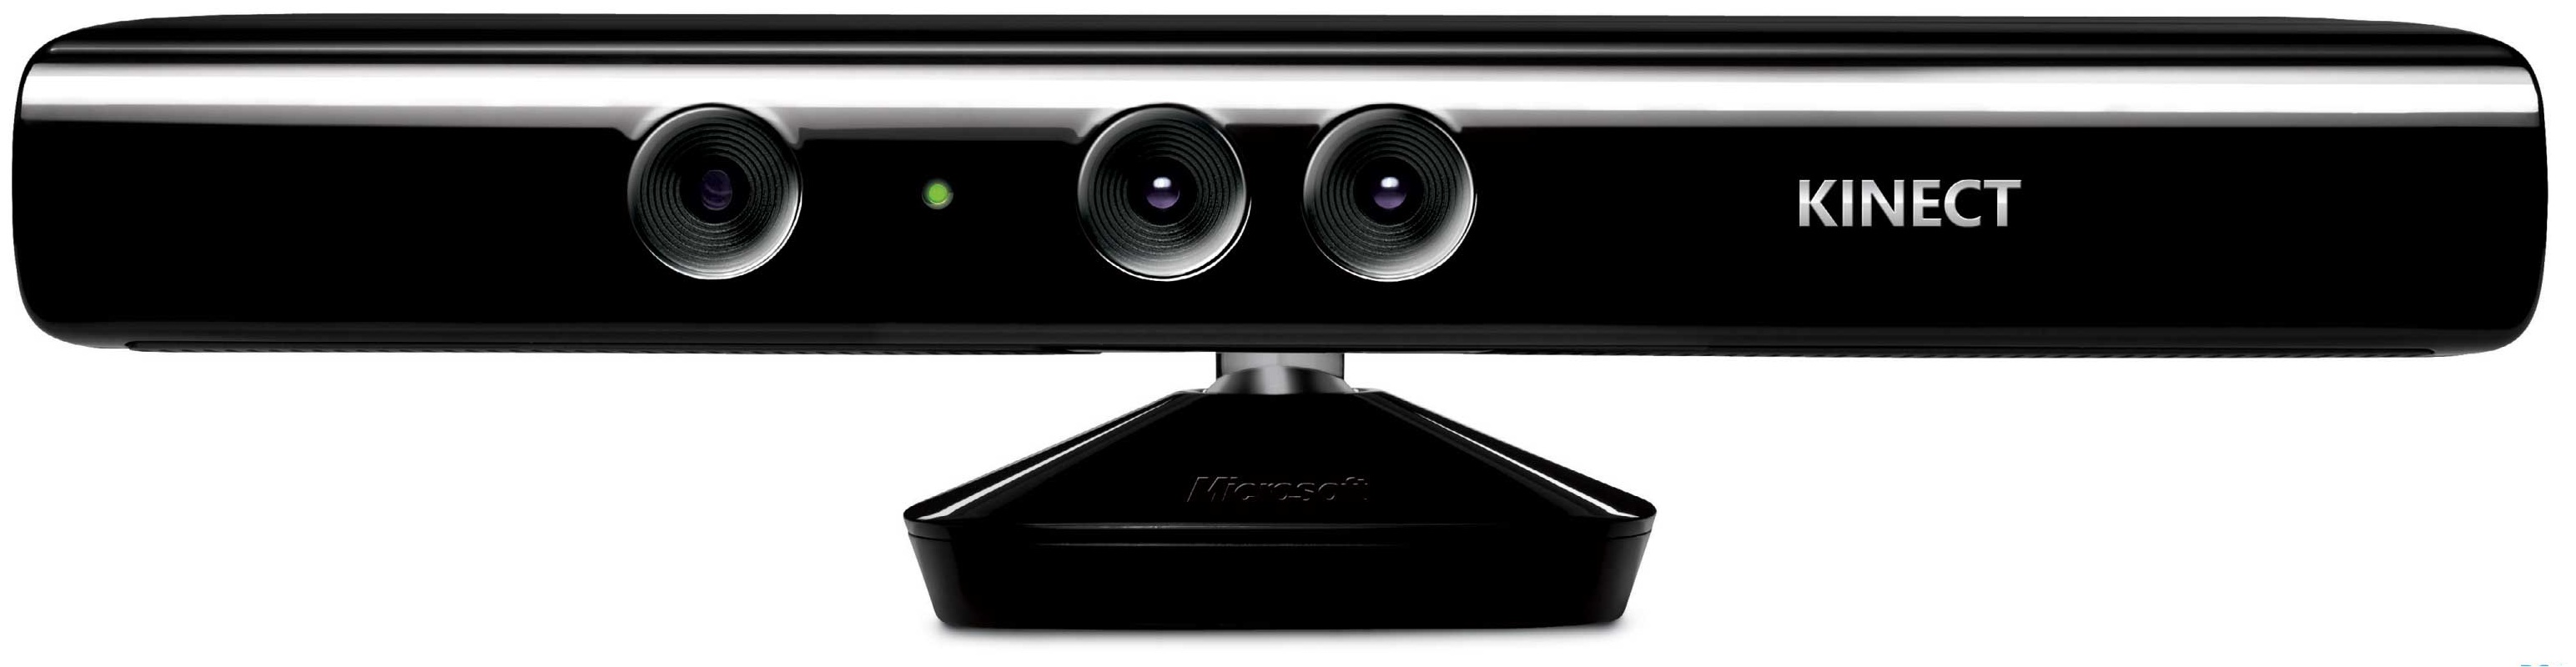
\includegraphics[width=\textwidth]{../figures/presentation/intro_kinect.jpeg}
  \end{center}
  \begin{itemize}
    \item 30 frames per second
    \item D - 9 million pixel values per second
    \item Algorithms must handle a high rate of data
  \end{itemize}

  \note{\begin{itemize}
    \item Kinect
    \item First affordable sensor to provide
    \item high resolution spatial information
    \item[]
    \item High rate of data
    \item Algorithms must have this as a design consideration
  \end{itemize}}
\end{frame}

\subsection{Map}

\begin{frame}{Mesh} % __________________________________________________
  \begin{center}
    \includegraphics[width=\textwidth]<1>{../figures/presentation/intro_mesh.png}
  \end{center}
  \only<2>{
  \vspace{-0.5in}
  \begin{itemize}
    \item Supported
    \item Computationally Inexpensive
    \item Low Memory Requirement
  \end{itemize}
  }

  \note<1>{\begin{itemize}
    \item There are different types of maps
    \item Mesh is the map type chosen for this work
  \end{itemize}}
  \note<2>{\begin{itemize}
    \item Supported
    \item - available software, tools, research, algorithms, etc., for
    this type of map
    \item Computationally Inexpensive
    \item - GPUs make this computationally efficient
    \item Low Memory Requirement
    \item - Can it run on a laptop with a standard amount of RAM?
  \end{itemize}}
\end{frame}

\subsection{Contribution}

\begin{frame}{Pipeline} % ______________________________________________
  \hspace*{-12.5mm}
  \includegraphics[width=1.2\textwidth]<1>
    {../figures/intro_general_pipeline_blackbox.pdf}
  \includegraphics[width=1.2\textwidth]<2>
    {../figures/intro_general_pipeline_mabdi.pdf}

  \note<1>{\begin{itemize}
    \item Traditional Mesh-Based Mapping Methods
    \item - Take incoming data
    \item - Generate a mesh structure
    \item - Append to growing global mesh structure
  \end{itemize}}

  \note<2>{\begin{itemize}
    \item MABDI
    \item - Takes what we already know
    \item (the global mesh structure)
    \item - Uses it to throwaway points in the data that are redundant
    \item Ability to classify incoming data and only use what is novel
    \item is MABDI's contribution
  \end{itemize}}
\end{frame}

\begin{frame}{Contribution} % ______________________________________________
  MABDI's algorithmic design identifies redundant information and removes it
  \emph{before} it is added to the global mesh.
\end{frame}


\section{Approach}

% Algorithmic Design

\begin{frame}{Variables} % ____________________________________________________

Description of the main variables

  \begin{table}[h]
    \begin{center}
      \begin{tabular}{c|l}
      \cellcolor{white} Variable Name & Description \\ % adding \cellcolor{} here fixes the vertical line between the columns for some reason
      \rowcolor{LightGray}
      $D$ & Depth image from RGB-D sensor \\
      $P$ & Pose of the sensor \\
      \rowcolor{LightGray}
      $D_n$ & Parts of $D$ that are \emph{novel} \\
      $S$ & Novel surface generated from $D_n$ \\
      \rowcolor{LightGray}
      $M$ & Global mesh \\
      \end{tabular}
    \end{center}
  \end{table}

\end{frame}

\note[itemize]{
\item Before we begin, let us get familiar with common variable names.
}


\begin{frame}{MABDI Algorithm} % _______________________________________________
  \vspace{-0.15in}
  \begin{center}
  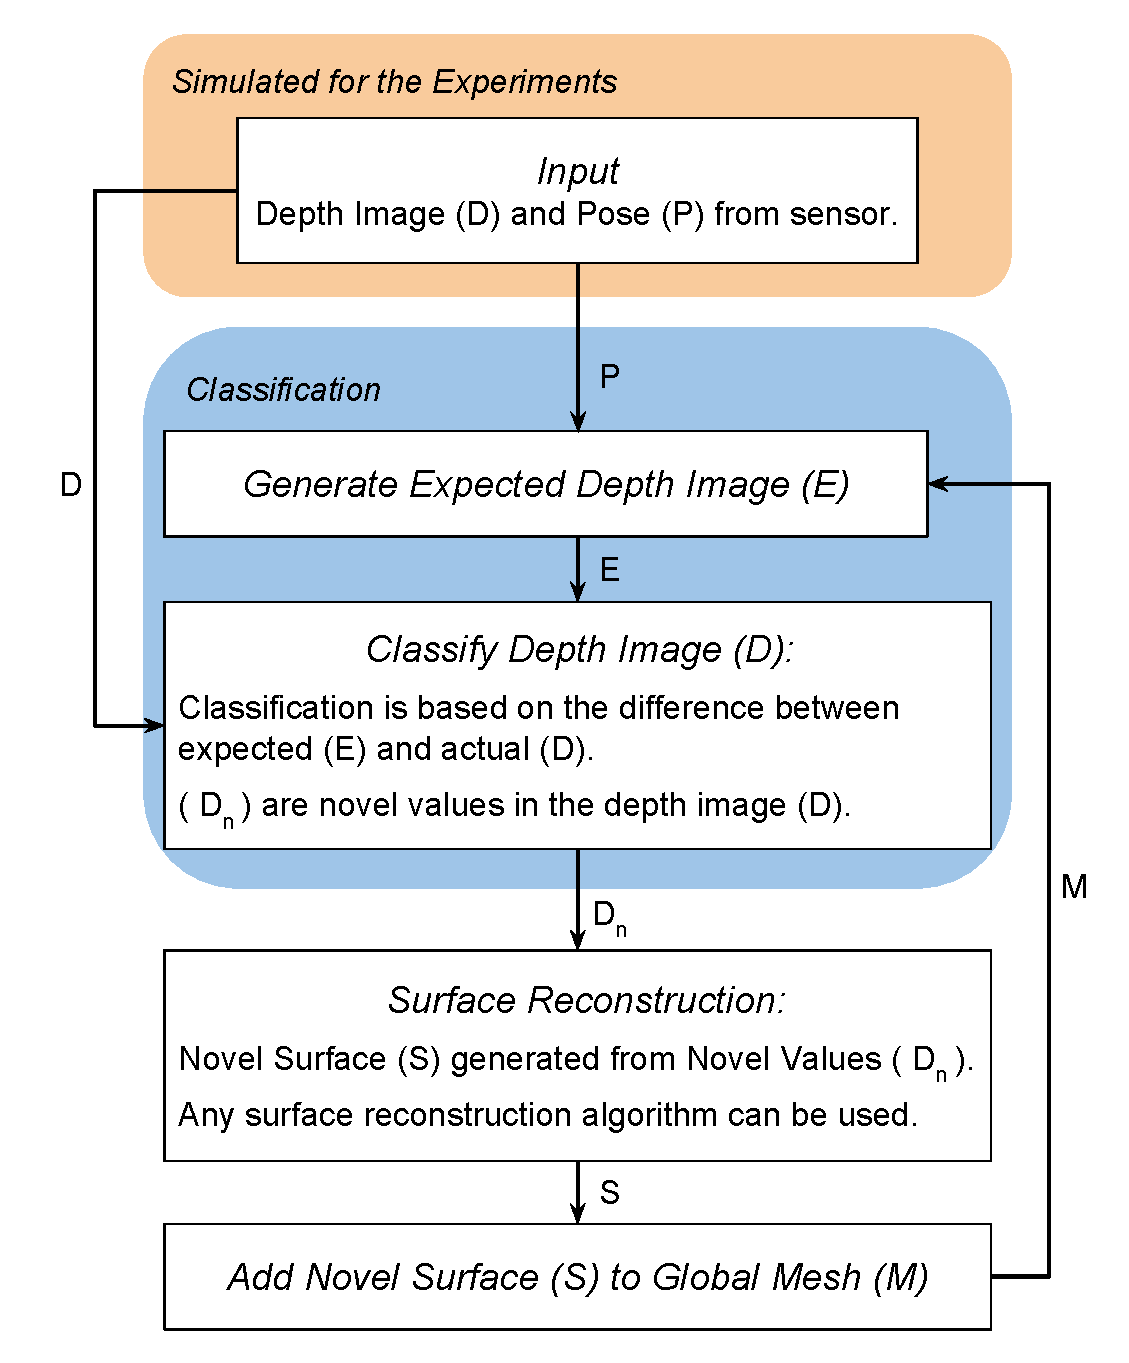
\includegraphics[height=0.95\textheight]{../figures/approach_mabdi_algorithm.pdf}
  \end{center}
\end{frame}

\note[itemize]{
\item[] Input
\item Has been simulated for this work
\item Cover in detail in next section
\item[] Generate Expected Depth Image
\item What we expect to see from our sensor
\item[] Classify Depth Image
\item Determine which points from D are novel
\item[] Surface Reconstruction
\item Create a mesh structure from the novel points
\item Cover in detail next
}

\subsection{Implementation}

% Surface Reconstruction

\begin{frame}{Topology Defined on Depth Image} % _______________________________
\begin{center}
  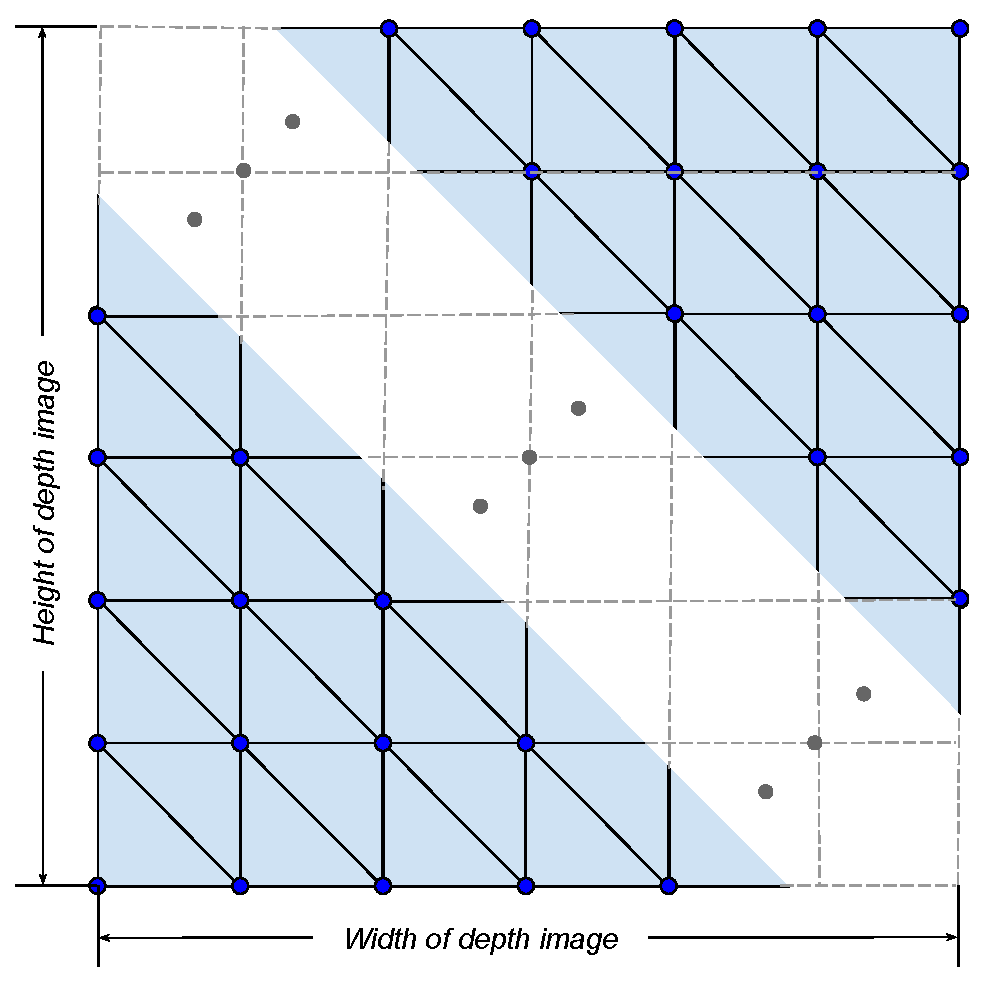
\includegraphics[height=0.90\textheight]{../figures/approach_sr_topology.pdf}
  \end{center}
\end{frame}

\note[itemize]{
\item Mesh consists of vertices and elements
\item - Vertices are points
\item - Elements define connections between vertices
\item Depth image
\item - Not a set of unorganized points
\item - Has structural information
\item - This allows us to define a topology in 2D that is preserved when projected to 3D
}

\begin{frame}{Removing elements} % _____________________________________________
  Elements are removed from the $S$ if they touch pixels from the sets:
  \begin{itemize}
    \item $D_{known}$
    \item $D_{boundary}$
    \item $D_{invalid}$
  \end{itemize}
  % TODO: Venn diagram
\end{frame}

\begin{frame}{Removing elements - $D_{known}$} % _______________________________
  \begin{gather*}
    D_n = \lvert D - E \rvert > threshold \\
    D_{known} = D \setminus D_n
  \end{gather*}
\end{frame}

% Software Design

\begin{frame}{Removing elements - $D_{boundary}$} % ____________________________
  \begin{gather*}
    K = \begin{bmatrix} 2 & -1 \\ -1 & 0 \end{bmatrix} \\
    D_{boundary} = (D \ast K) > threshold
  \end{gather*}
\end{frame}

\note[itemize]{
\item
}

\begin{frame}{Removing elements} % _____________________________________________
  \begin{center}
  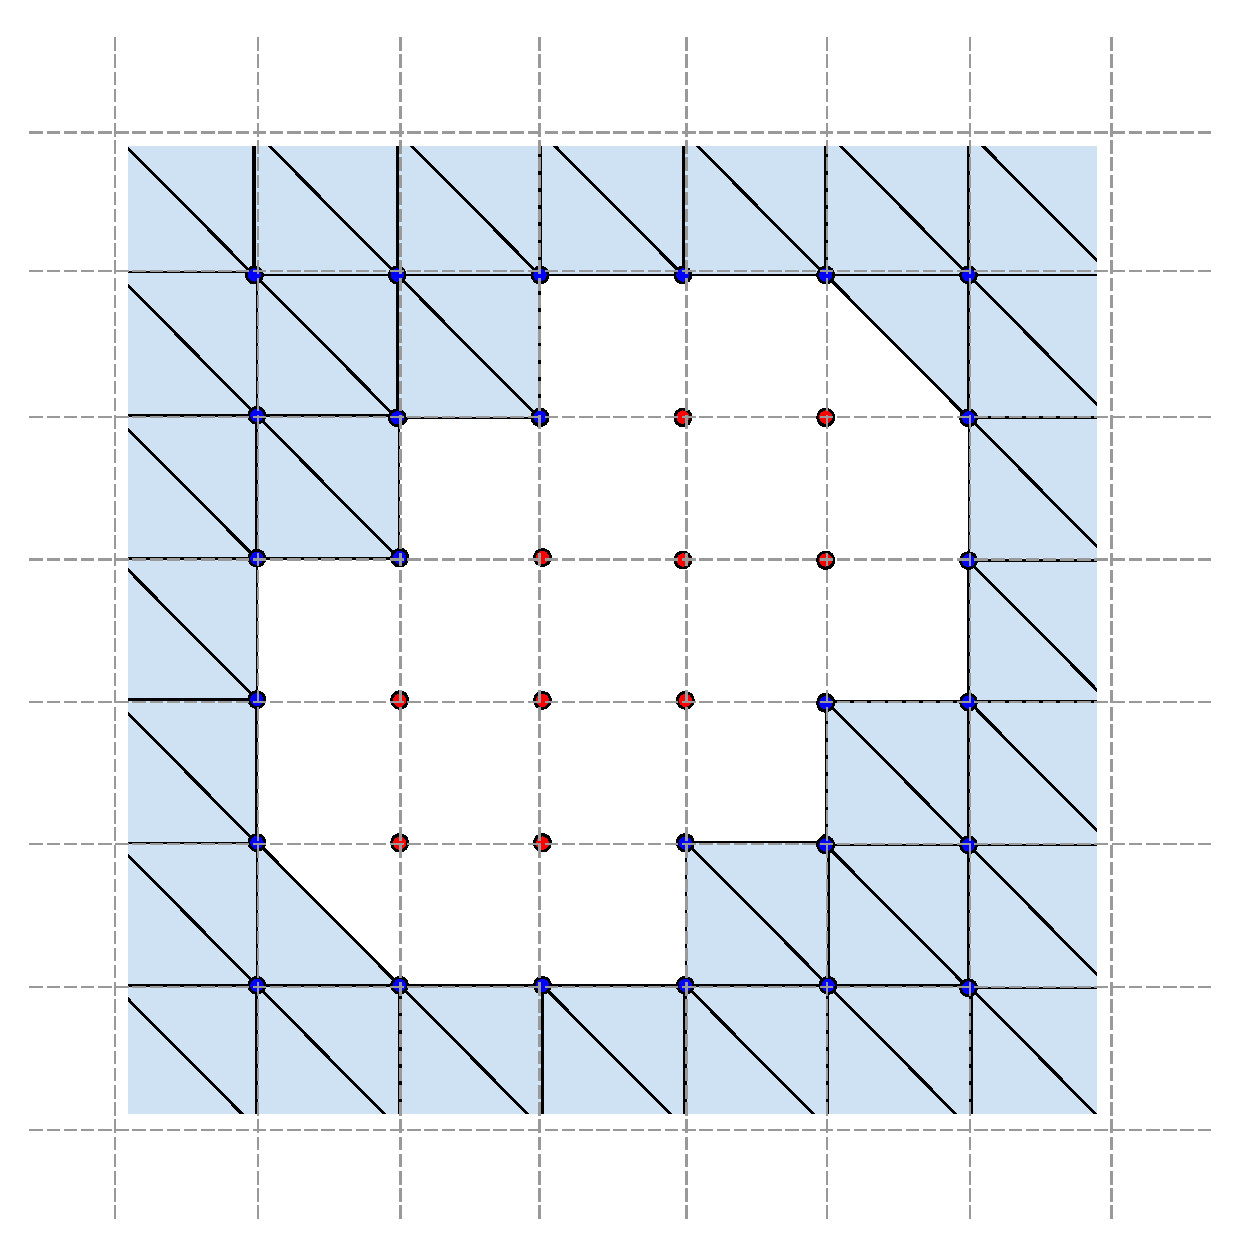
\includegraphics[height=0.90\textheight]{../figures/approach_sr_element_removal.pdf}
  \end{center}
\end{frame}

\note[itemize]{
\item
}

\subsection{Software Design}

\begin{frame}{Diagram} % _______________________________________________________
  \begin{center}
  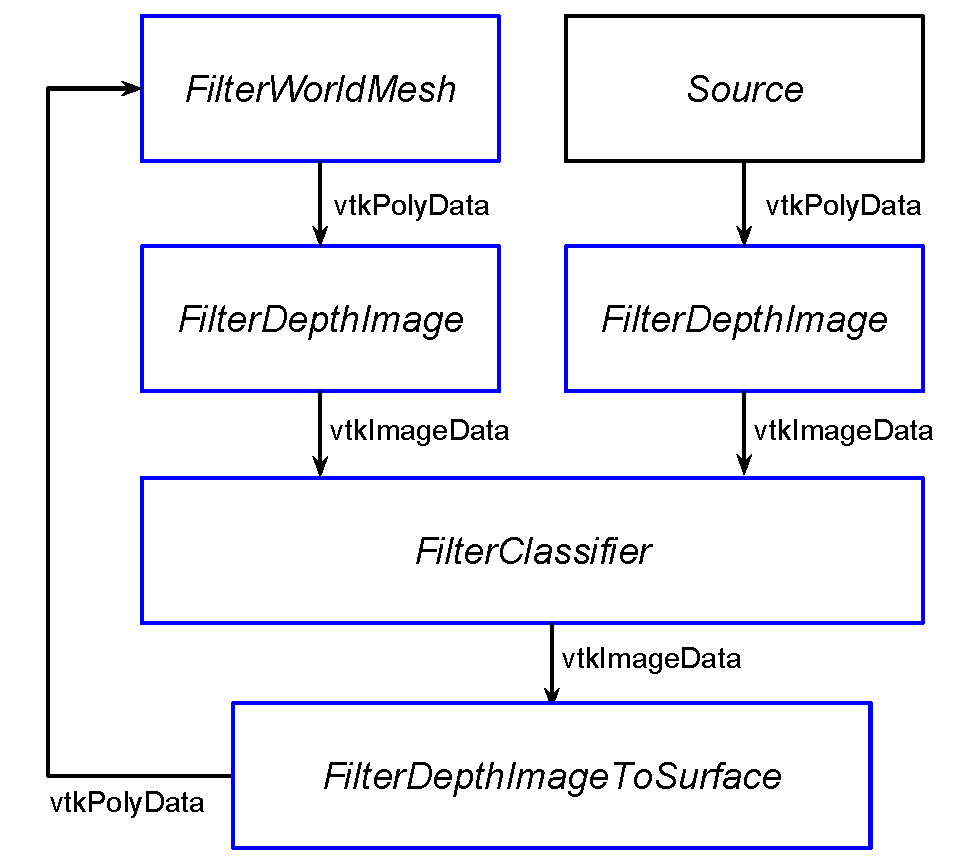
\includegraphics[height=0.90\textheight]{../figures/approach_software_diagram.pdf}
  \end{center}
\end{frame}

\note[itemize]{
  \item  \textit{Source} - Classes with the prefix Source define the
  environment that is used for the simulation and provide a mesh in the form
  of a vtkPolyData.
  \item \textit{FilterDepthImage} - Render the incoming vtkPolyData in a
  window and output the depth buffer from the window as a vtkImageData. The
  output additionally has pose information of the sensor.
  \item \textit{FilterClassifier} - Implements the true innovation of MABDI,
  i.e., takes the difference between the two incoming depth images
  (vtkImageData) and outputs a new depth image where the data that is not
  novel is marked to be thrown away.
  \item \textit{FilterDepthImageToSurface} - Performs surface reconstruction
  on the novel points. The surface is output as a vtkPolyData.
  \item \textit{FilterWorldMesh} - Here we simply append the incoming novel
  surface to a growing global mesh that is also output as a vtkPolyData.
}


\section{Experimental Setup}

\subsection{Simulation Overview}

\begin{frame}{Overview} % _____________________________________________
  \begin{center}
  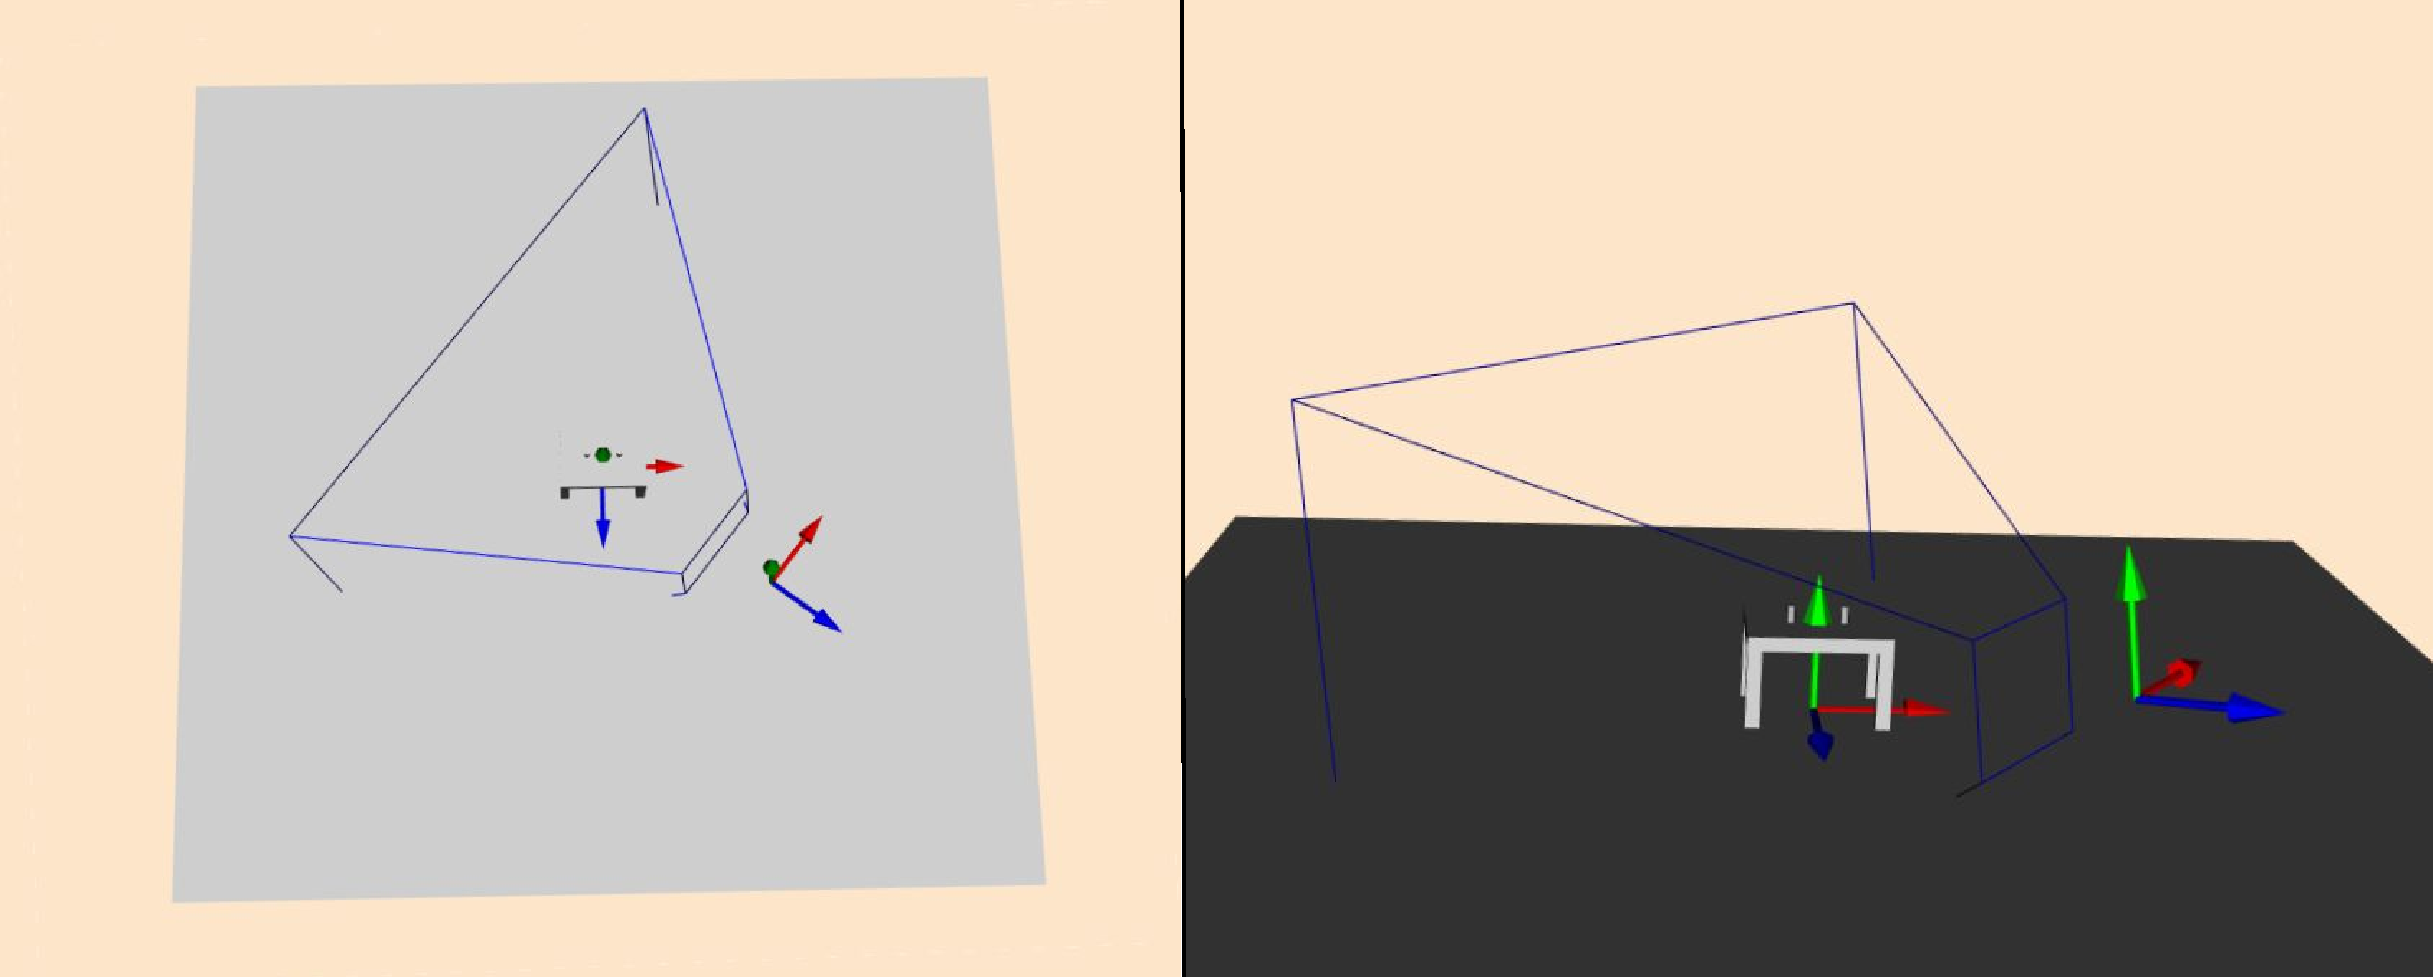
\includegraphics[width=\textwidth]
    {../figures/expsetup_simulation_overview.pdf}
  \end{center}
\end{frame}

\note[itemize]{
\item
}

\subsection{Simulating a RGB-D Sensor}

\begin{frame}{Rendering Pipeline} % ____________________________________________
  \begin{center}
  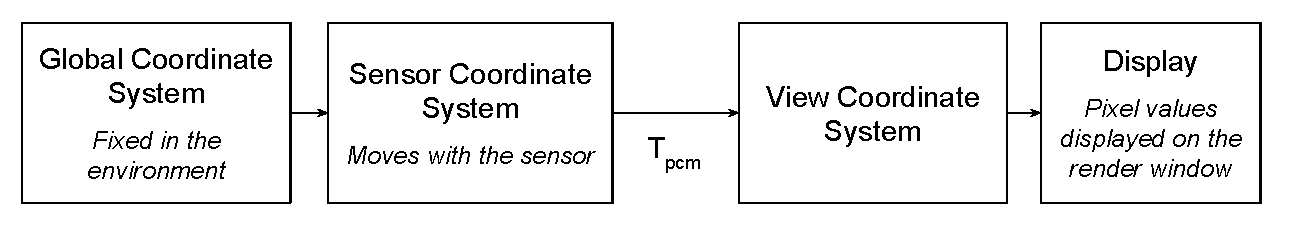
\includegraphics[width=\textwidth]
    {../figures/expsetup_render_pipeline.pdf}
  \end{center}
\end{frame}

\note[itemize]{
\item Render pipeline: projects 3D global coordinates to 2D pixel coordinates
}

\begin{frame}{$T_{pcm}$} % _____________________________________________________
  \vspace{-0.15in}
  \begin{center}
  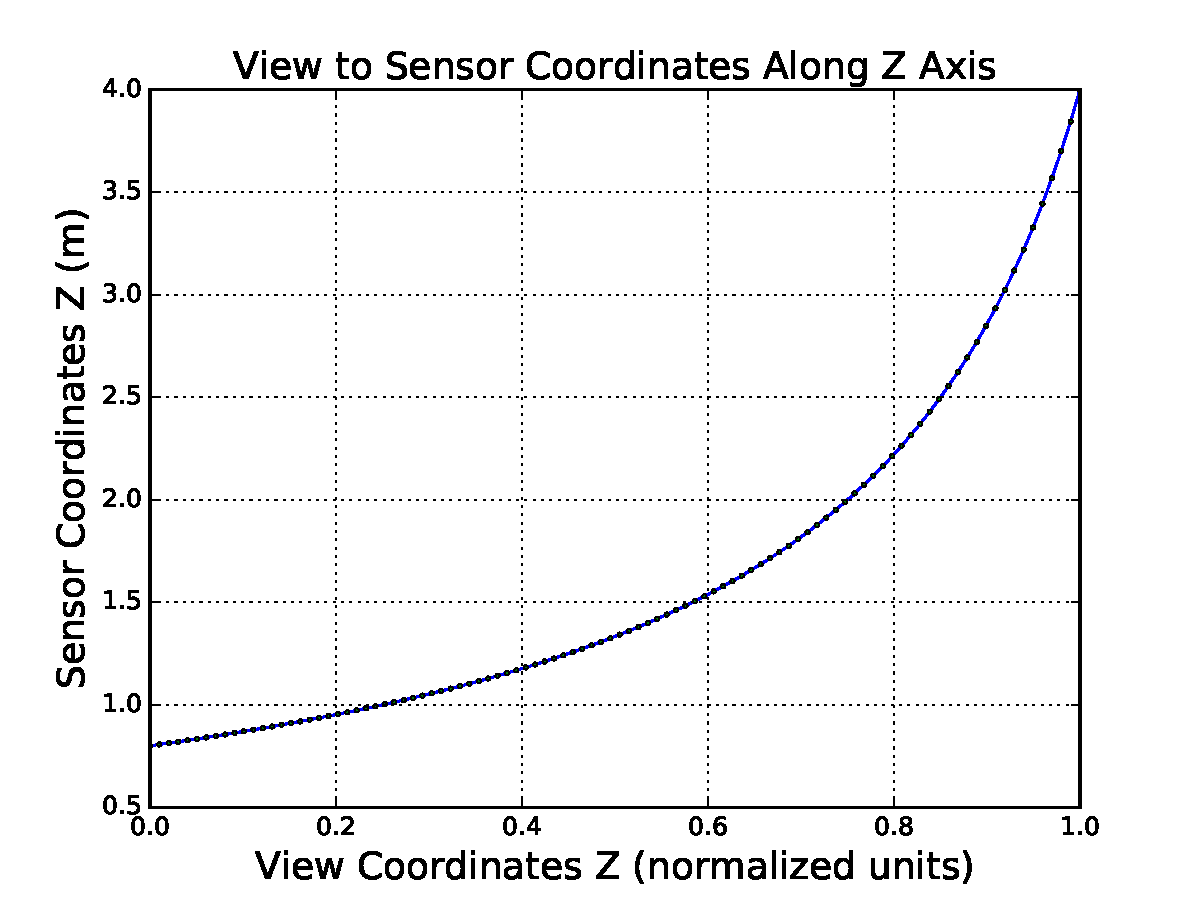
\includegraphics[height=0.90\textheight]
    {../figures/expsetup_depth_view_to_sensor.pdf}
  \end{center}
\end{frame}

\note[itemize]{
\item The pinhole camera transformation, $T_{pcm}$, creates a non-linear
relationship between values in the depth image and their corresponding location
in the sensor's coordinate system.
}

\begin{frame}{Adding Noise} % __________________________________________________
  \vspace{-0.15in}
  \begin{center}
  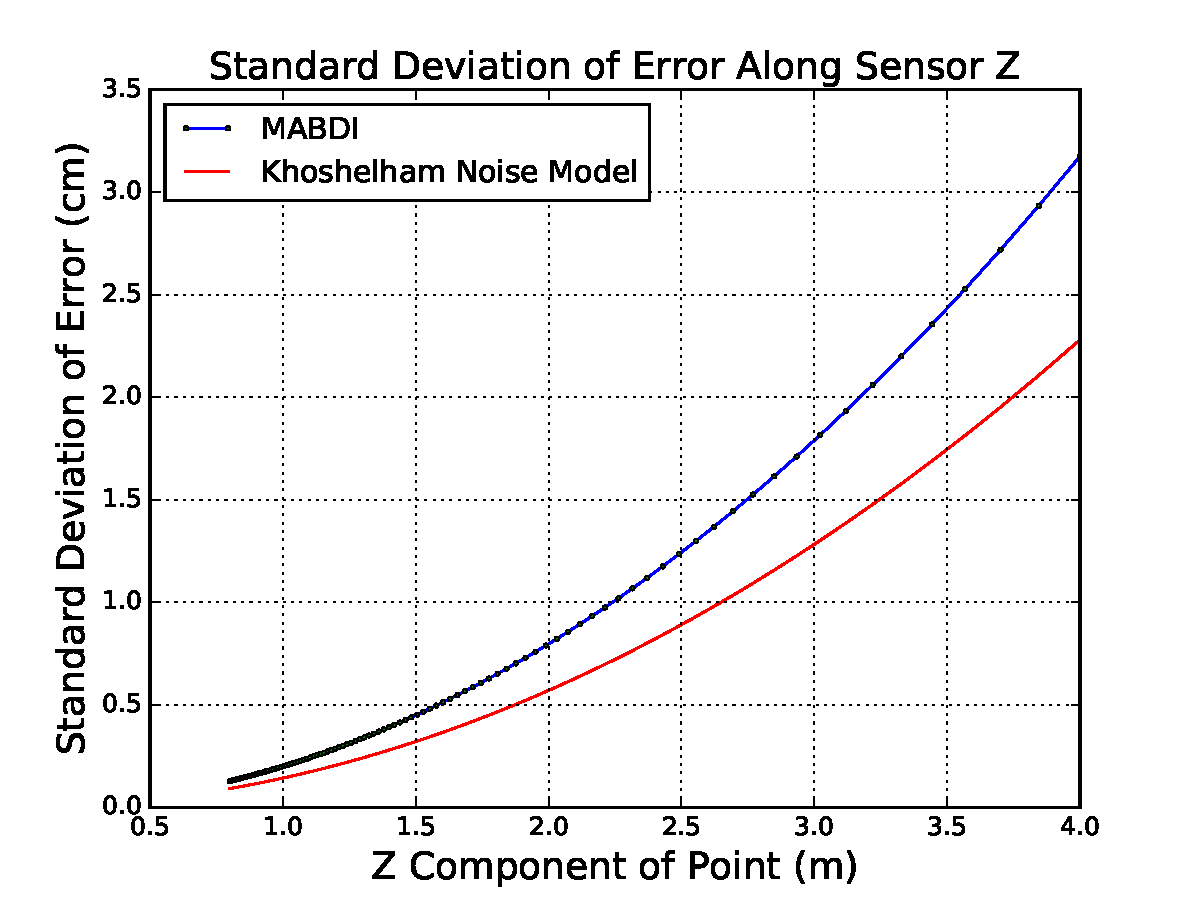
\includegraphics[height=0.90\textheight]
    {../figures/expsetup_noise_error.pdf}
  \end{center}
\end{frame}

\note[itemize]{
\item Comparison of standard deviation of the error used in the MABDI simulation and the error model from Khoshelham.
}

\subsection{Sensor Path}

\begin{frame}{Sensor Path} % __________________________________________________
  \vspace{-0.15in}
  \begin{center}
  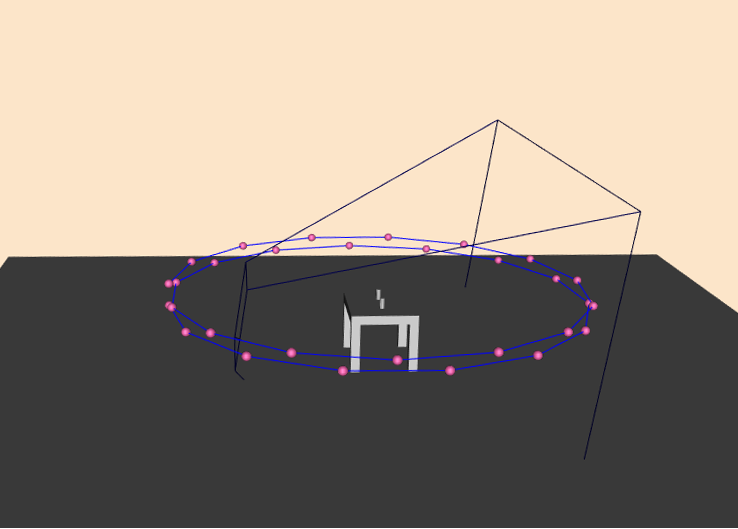
\includegraphics[height=0.90\textheight]
    {../figures/expsetup_path.png}
  \end{center}
\end{frame}

\note[itemize]{
\item The blue line indicates the path and the pink points indicate where the
sensor stops along the path. The path circles the objects in the environment
twice. A helical path was chosen because it returns to a part of the environment
that has already been mapped and is thus ``known'' to the algorithm. Also,
because the path is a helix and not just a circle, the sensor views the
environment from a slightly different position on each pass.
}

\subsection{Simulation Parameters}

\begin{frame}{Simulation Parameters} % _________________________________________
  \begin{table}[h]
    \begin{center}
      \begin{tabular}{|l|c|c|c|c|}
      \hline
             & Environment & Noise   & Dynamic & Iterations \\\hline
      Run 1	 & Table       & False   & False   & 30 \\
      Run 2  & Bunnies     & True    & False   & 50 \\
      Run 3  & Bunnies     & True    & True    & 50 \\
      \hline
      \end{tabular}
    \end{center}
  \end{table}
\end{frame}

\note[itemize]{
\item Environment - This parameter specifies the environment used to generate
the simulated depth images. \textit{Table} is an environment consisting of a
table and two cups placed on the table. The table is 1 meter tall.
\textit{Bunnies} is an environment consisting of three bunnies that are
around 1.5 meters tall. These bunnies are created using the Stanford Bunny a well known data set in computer graphics.
\item Noise - If true, adds noise to the depth image of the simulated sensor.
\item Dynamic - If true, adds an object during the simulation. In the case
of this analysis, a third bunny is added half-way through the simulation.
\item Iterations - The number of times MABDI will run. This number is equal to the number of stops the sensor makes along the path because every time the sensor stops MABDI is run to update the global mesh.
}


\section{Results}

\begin{frame}{During the Experiment} % _________________________________________
  \vspace{-0.15in}
  \hspace*{-12.5mm}
  \includegraphics[width=1.2\textwidth]<1>
    {../figures/results_run2_novel_portion.png}
  \includegraphics[width=1.2\textwidth]<2>{../figures/results_run2.pdf}
  \includegraphics[width=1.2\textwidth]<3>{../figures/results_run3.pdf}

  \note<1>{\begin{itemize}
    \item Novel portion of the environment.
    \item To be discussed during Experiment 2.
  \end{itemize}}

  \note<2>{\begin{itemize}
    \item[] Yellow portion is the entirety of $M$ after the first iteration
    \item Due to occlusion, novel portion not represented
    \item[] Sensor sees portion on this iteration
    \item[] We don't expect to see portion (not in $M$)
    \item classification process successfully identifies (highlighted by a red circle)
    \item[] Novel surface $S$ now represents the novel portion
    \item Finally
    \item novel portion is represented by the global mesh $M$.
  \end{itemize}}

  \note<3>{\begin{itemize}
    \item Bunny added during this iteration
    \item $D$ shows the new bunny
    \item $E$ does not show the new bunny
    \item classification process successfully identifies
    \item novel points are used to generate the novel surface $S$
    \item $S$ is appended to $M$
    \item[] $S$ has large number of elements for this particular iteration
    \item plot shows resulting jump in the number of elements contained with $M$  \end{itemize}}
\end{frame}

\begin{frame}{Mesh Quality} % ______________________________________________
  \vspace{-0.15in}
  \hspace*{-12.5mm}
  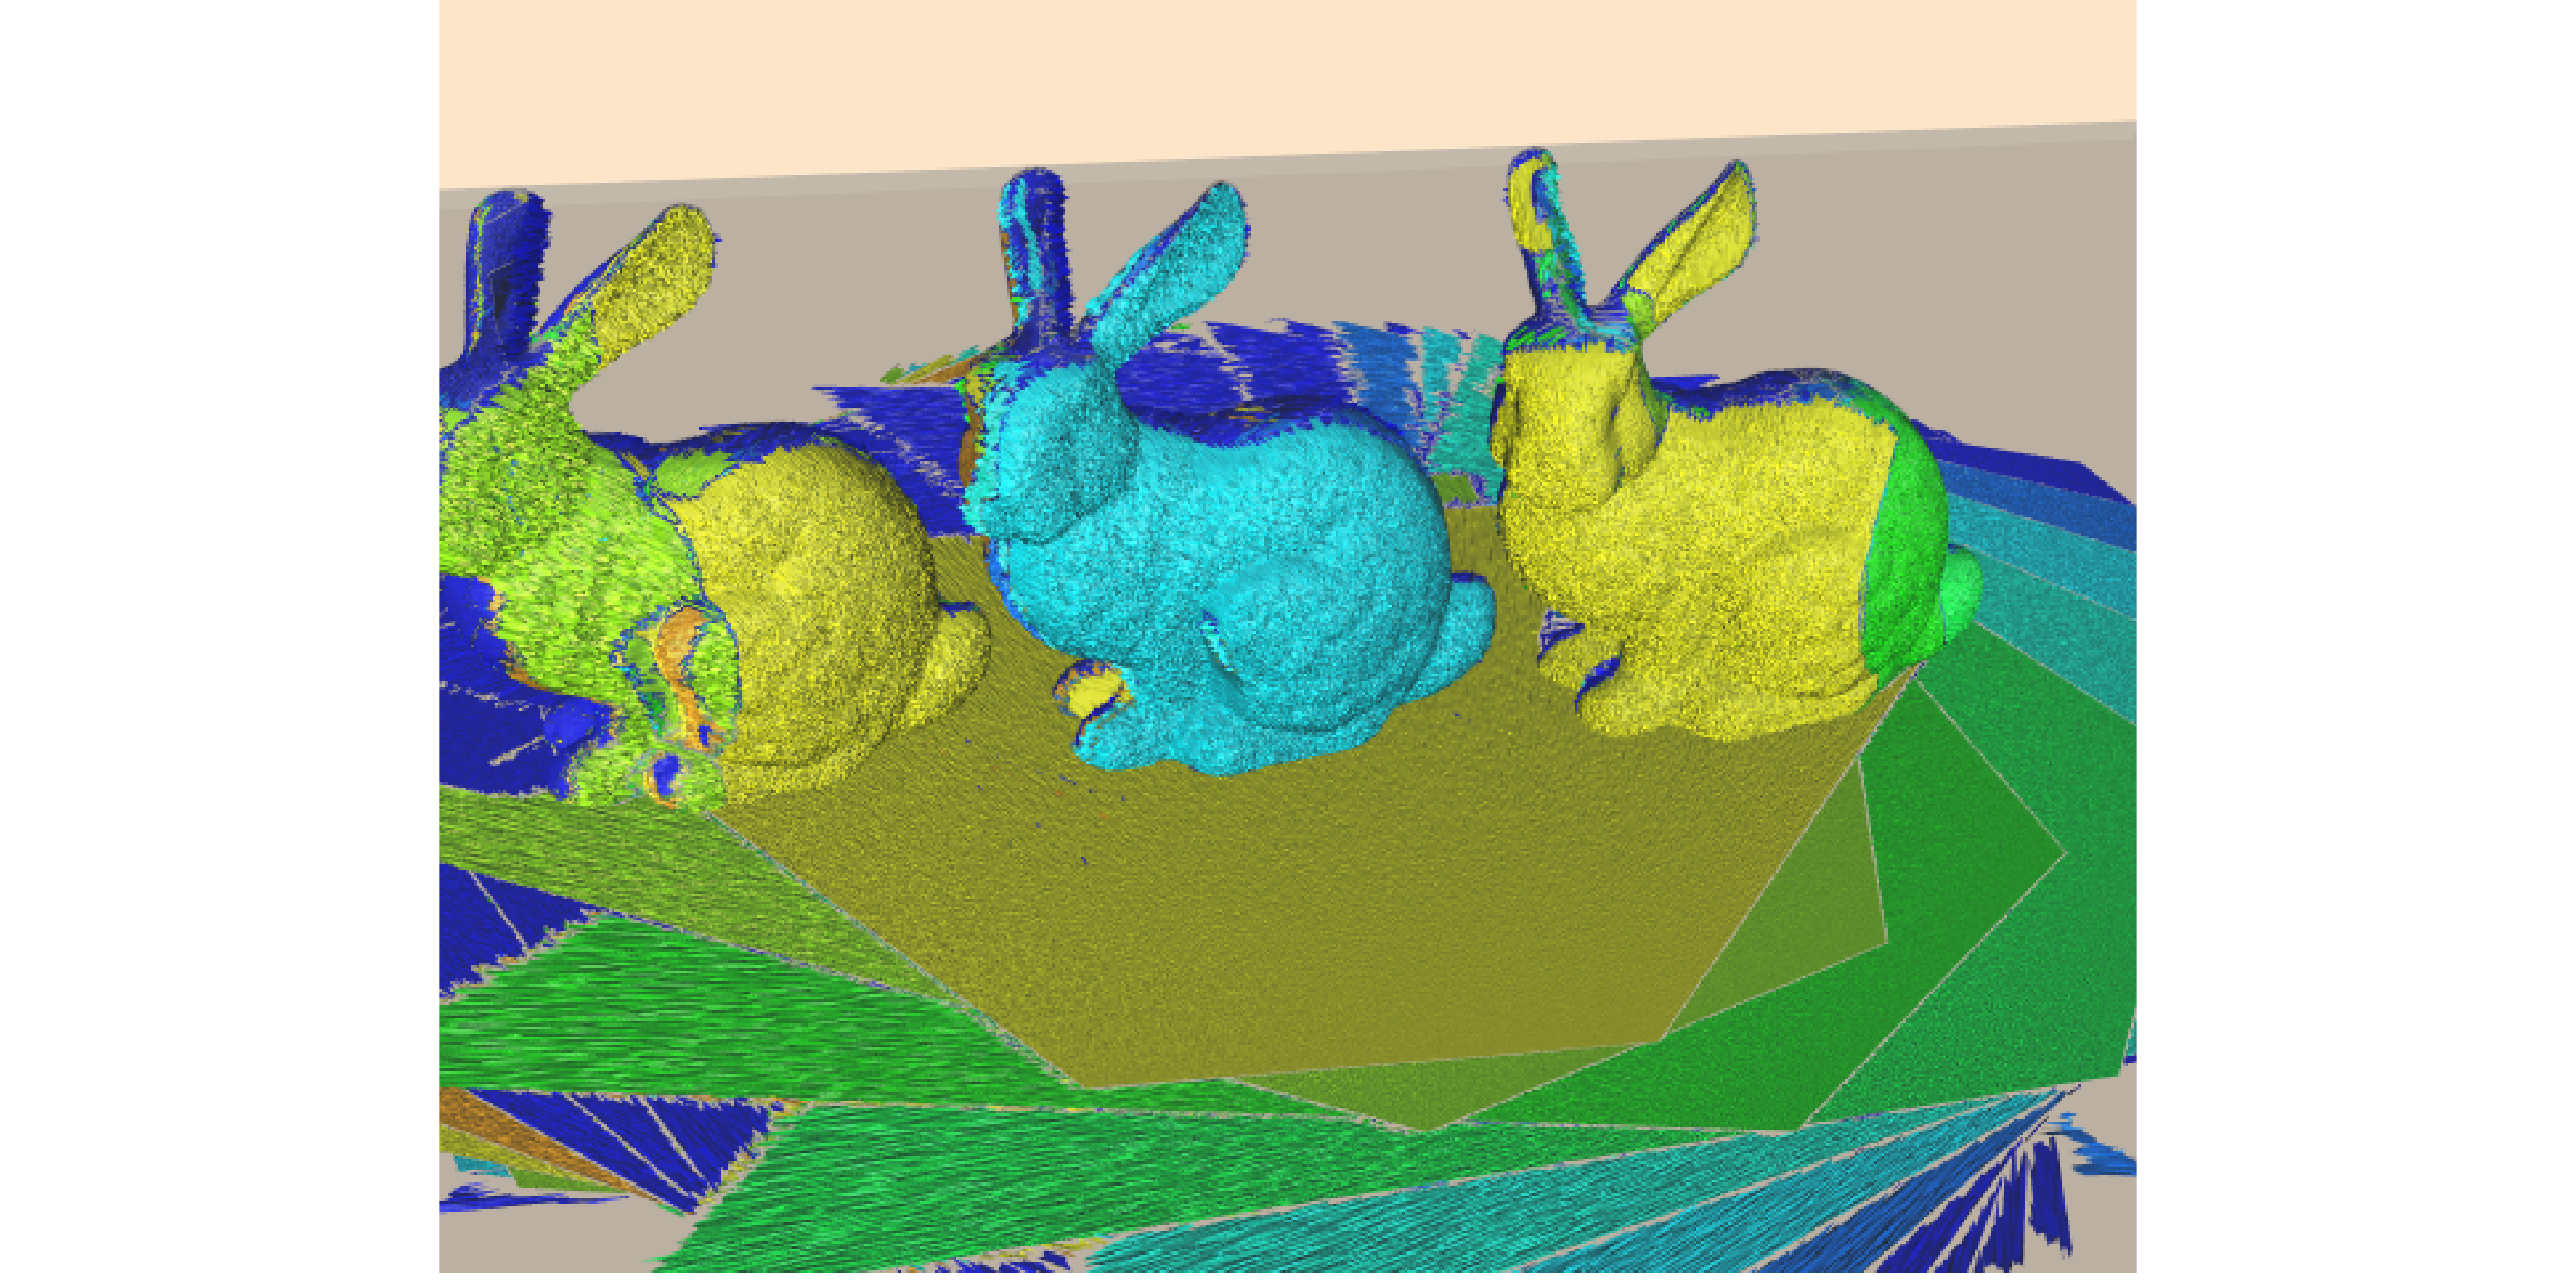
\includegraphics[width=1.2\textwidth]{../figures/results_run3_global_mesh.png}

  \note<1>{\begin{itemize}
    \item Gaps in the mesh
    \item - Traditional methods have overlapping layers
    \item - So you don't notice gaps
    \item The mesh is noisy.
    \item - Our method simply connects
    neighboring points in the point cloud without additional steps such as
    Laplacian smoothing
    \item[]
    \item My reconstruction method was sufficient for demonstrating the
    usefulness of the MABDI algorithm
    \item - mesh has the same magnitude of noise as the sensor's simulated noise
  \end{itemize}}

\end{frame}

\begin{frame}{Mesh Progression} % ______________________________________________
  \vspace{-0.15in}
  \hspace*{-12.5mm}
  \includegraphics[width=1.2\textwidth]<1>{../figures/results_run1_gm.pdf}
  \includegraphics[width=1.2\textwidth]<2>{../figures/results_run2_gm.pdf}
  \includegraphics[width=1.2\textwidth]<3>{../figures/results_run3_gm.pdf}

  \note<1>{\begin{itemize}
    \item[] Traditional methods
    \item would have a plot similar to that indicated by the red arrow on the graph
    \item[] MABDI
    \item levels off as the environment becomes more known
  \end{itemize}}

  \note<2>{\begin{itemize}
    \item MABDI is reactive as the sensor moves to parts of the environment that
    are rich in information
    \item the mesh grows rapidly based on the needs of the environment
  \end{itemize}}

  \note<3>{\begin{itemize}
    \item Large jump in graph corresponding to new bunny
  \end{itemize}}
\end{frame}


\section{Conclusion}

\begin{frame}{Motivation} % ____________________________________________________
  The goal of MABDI is to identify data from the sensor that has not yet been
  represented in the map and use this data to add to the map. MABDI does this by
  leveraging the difference between what we are actually seeing and what we expect
  to see. MABDI can work in conjunction with any current mesh-based surface
  reconstruction algorithms, and can be thought of as a general means to provide
  introspection to those types of reconstruction methods.

  The MABDI implementation was able to successfully perform in a realistic
  simulation environment. The results show how novel sensor data was
  successfully classified and used to add to the global mesh. Also, the MABDI
  algorithm runs at around 2Hz on a consumer grade laptop with an Intel i7
  processor. This performance means that it is capable of real-world
  applications.

  Currently MABDI is only designed to handle object addition, but the idea can be
  extended to handle both object addition and removal as discussed in Section
  \ref{section:algorithmic_design}. This would give the system the
  capability to handle highly dynamic environments such as a door opening and
  closing.
\end{frame}


\end{document}
